\documentclass{standalone}

\begin{document}

\section[CHIMeRA as a Service]{CHIMeRA as a Service}\label{chimera:caas}

We have discussed about the information stored into \textsf{CHIMeRA} database, but we have ignored how we could manage these data.
More than the realization of a useful database, we have to provide an easy-to-use interface to encourage the research community to manage our processed information.
We have already discussed about how modern databases are shared along the Internet and how these large quantities of data could be handled using database languages (ref. \ref{chimera:chimera}).
Now we have to find the best solution for our application.

We developed a first version of \textsf{CHIMeRA} database using \textsf{SQL} (\emph{Structured Query Language}) language\footnote{
  \textsf{SQL} is a domain-specific language designed for managing data held in a relational database management system (RDBMS) and it is particularly efficient in handling structured data.

} and in particular the \href{https://www.sqlite.org/index.html}{\textsf{SQLite}} one.
\textsf{SQLite} is probably the easier solution for database management and the creation of efficient queries is straightforward.
It is a well performing solution for standard relational databases, but it does not provide any facility for network structures.
Moreover, \textsf{SQLite} is not directly comparable to client/server \textsf{SQL} database engines such as \textsf{MySQL}, \textsf{Oracle}, \textsf{PostgreSQL} or \textsf{SQL Server} since it is designed only for local data storage and individual applications.
It is extremely efficient and simple in its applications but it does not cover the requirements posed by our \textsf{CHIMeRA} structure and our needs about sharing information.

\begin{figure}[htbp]
\centering
\def\svgwidth{0.8\textwidth}
\input{./img/arango_perf.pdf_tex}
\caption{\textsf{NoSQL} Performance Benchmark 2018 (source \href{https://www.arangodb.com/2018/02/nosql-performance-benchmark-2018-mongodb-postgresql-orientdb-neo4j-arangodb/}{here}).
Absolute \& normalize results for \textsf{ArangoDBD}, \textsf{MongoDB}, \textsf{Neo4j} and \textsf{OrientDB}.
Comparison of time-performances using different (common) \textsf{NoSQL} queries.
The first row shows the computing time on different \textsf{NoSQL} queries using \textsf{ArangoDB}.
We mark with green boxes the solutions which perform better than \textsf{ArangoDB} and with red boxes the worse.
}
\label{fig:arango}
\end{figure}

A more efficient solution is provided by modern graph databases (GDB).
GDBs are databases which use graph structures to represent and store information: there are two needed information for the database given by nodes and edges.
The key concept behind this kind of storage is the relationship between entries.
They go under the \textsf{NoSQL} (\emph{not SQL}, or better \quotes{\emph{Not only SQL}}) database category, which store data according to more sophisticated models than simple tabular relations (typical model of \textsf{SQL} databases).
GDBs allow simple and efficient retrieval of complex hierarchical structures by definition, representing the most efficient solution for our \textsf{CHIMeRA} database which is born as a network-of-networks architecture.
Several solutions have been proposed to address graph storages and there are a wide range of possible GDB languages publicly available on-line (e.g \textsf{Neo4j}, \textsf{OrientDB}, \textsf{Sparksee}, \textsf{AllegroGraph}, $\cdots$).
Based on our experience about these topics and driven by the available documentation (ref Fig.~\ref{fig:arango}), we have chosen to use \href{https://www.arangodb.com/}{\textsf{ArangoDB}} in our application.

\textsf{ArangoDB} is an open-source and free software released on Github for multi-model database management with a unified query language \textsf{AQL} (\emph{ArangoDB Query Language}).
\textsf{ArangoDB} database system is \textsf{NoSQL}, but its queries are very closed to \textsf{SQL} ones and, thus, they are easy to write also by no-expert users.
The code core is written in \textsf{C++} and, thus, it is extremely efficient from a numerical point-of-view (ref. Fig.~\ref{fig:arango}).
Moreover, it provides also a user-friendly web interface for network visualization and query development.
The possibility to have a web interface allows an easy way to share our database on Internet as a service, increasing the usability of our tool.
Moreover, query outputs can be also downloaded and used by external tools.
Thus, using \textsf{ArangoDB} as service manager we provide a \emph{Software as a Service} (SaaS) interface of our \textsf{CHIMeRA} database (\emph{CaaS}).
This project is still in work in progress and this CaaS is not yet publicly available\footnote{
  As soon as possible we intend to create it jointly to an adequate computational environment ables to support multiple external queries.
}.

We reformatted \textsf{CHIMeRA} network following the \textsf{ArangoDB} requirements and we created the graph database structure of our data.
Using this database we have been able to perform the first queries and discuss about the results.
The University of Bologna is currently involved into the \href{https://www.harmony-alliance.eu/}{HARMONY European project} for the analysis of hematological data provided by multiple pharmaceutical companies.
The HARMONY project aims to describe, analyze and model multiple the data collected by various partners, producing a personalized medicine framework for the study of hematological diseases.
This project is based on the harmonization of different databases in the same way as our \textsf{CHIMeRA} project aims to merge multiple public data sources.
The main focus of HARMONY project is on diseases related to different kinds of \emph{leukemia}.
\emph{Leukemia} is the most common type of cancer in children and it causes hundred of thousands of death every year.
It is an hematological disease and its exact causes are still unknown.
The developed \textsf{CHIMeRA} project could be used to contribute to this kind of researches, giving a wider biological overview about these diseases.
Thus, we decided to formulate our first query on the \emph{leukemia} disease.

We customized our query to extract only the 2nd neighbors related to this node.
The pseudo-code used for our query is shown in \ref{code:query}.

\lstset{style=Java}
\begin{lstlisting}[language=Java, caption=CHIMeRA 2nd neighbors query, label=code:query]
FOR x IN node_type_vertex
  FILTER x.name LIKE "looking_for_entry"
    FOR v, e, p IN 1..3 ANY x GRAPH "CHIMeRA"
      RETURN p
\end{lstlisting}

The query takes the node-collection (\textsf{ArangoDB} nomenclature) related to the searched node type (\textsf{node\_type\_vertex} in the code) and it filters all the names which satisfy the \textsf{LIKE} condition.
Starting from the found nodes, it returns the output graph preview made by the 1st and 2nd neighbors (range of values \textsf{1..3} in the code).

We applied this query-like looking for \emph{leukemia} node and we processed the results using \textsf{Gephi} as network viewer.
The obtained network is shown in Fig.\ref{fig:leukemia}: the network involves \numprint{9460} nodes and \numprint{26646} links.
As can be seen by the plot, just considering the 2nd neighbors the obtained subnetwork is quite large and it highlights the biological complexity of this disease.

\begin{figure}[htbp]
\centering
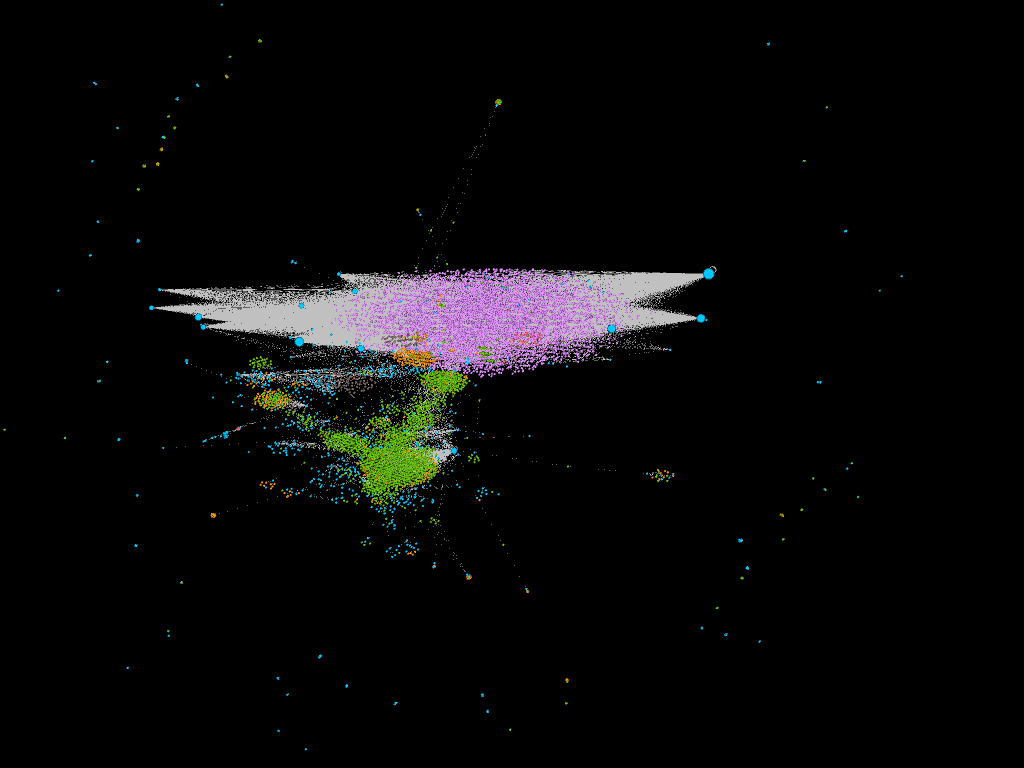
\includegraphics[width=.8\linewidth]{leukemia.png}
\caption{Output of \emph{leukemia} query obtained by \textsf{CHIMeRA} graph database using \ref{code:query}.
The subnetwork is made by the 2nd neighbors starting from all the nodes which include \quotes{leukemia} in their names.
The subnetwork includes 291 different types of leukemias clustered into 82 connected components.
The giant components is made by \numprint{9108} nodes.
\textsf{CHIMeRA} query is able to give a biomedical overview of the \emph{leukemia} diseases mapping 838 diseases, \numprint{2463} genes, 5195 SNPs, 154 metabolite pathways, 40 metabolites and 5 drugs associated to them.
}
\label{fig:leukemia}
\end{figure}

Using the \quotes{generic} name of \emph{leukemia} we found 291 different types of leukemia diseases into \textsf{CHIMeRA}, which denote different facets of this disease.
Despite these multiplicities of results, we noticed that they clustered in only 82 connected components, highlighting multiple similitudes between them.
In particular, we found a giant components of \numprint{9108} nodes and only other 6 components with more than 10 nodes.
The giant component includes 165 different facets of \emph{leukemia} disease, while the other connected components describe the remaining ones.
The powerful of \textsf{CHIMeRA} network born exactly from the analysis of these cases, where we can infer missing information starting from the knowledge about analogous researches given by the full set of information related to the giant component found.
In the giant component we can appreciate a description of the \emph{leukemia} disease given by all the other node types: we have 587 diseases, 4 drugs, 2409 genes, 40 metabolites, 154 metabolite pathways, 5195 possible phenotypes and 719 SNPs related to them.
The diseases associated to \emph{leukemia} can help to highlight possible analogies (co-morbidities) between this \quotes{difficult} disease and \quotes{easier} ones (cause and related disease connections) or simply provide a bridge to other node types (e.g drugs or genes) which are not directly related to the \emph{leukemia} using databases individually.
We would stress that, despite the \emph{phenotype} node-type which includes the more general biological information, all the other amount of node-types represent only a small percentage of the available information (disease 0.9\%, drug 0.01\%, gene 12.8\%, metabolite 0.03\%, pathway 11.5\%, SNP 0.6\%, phenotype 39.3\%).
It is important to monitor also this kind of percentages because they could bring to possible biases in our description.
A such biomedical overview could not be found using single-database approach and, to the best of the author's knowledge, only the \textsf{CHIMeRA} database is capable to map them.

The subnetwork extracted has more than half nodes as pendants (\numprint{5270}/\numprint{9108} or 57\%), i.e with degree score equal to $1$.
We have already discussed about this feature of \textsf{CHIMeRA} and, also in this case, we can use this behavior to connect other (possible) kinds of information to improve our disease description.
We are still working on the analysis of the extracted information and, especially, about their biomedical interpretation related to the \emph{leukemia} disease.
Moreover, we have to see how we can combine our data to the HARMONY project samples.
Thus, we end this chapter remarking the potential applications of a such network-of-networks structure and its capability of give us a more global overview of biomedical compounds in scientific researches.

\end{document}
